\documentclass[12pt]{article}

% a template that a friend gave, it's worked well enough for me
% i have added some packages and stuff that have proved useful

\usepackage{fancyhdr}
\usepackage{tipa}
\usepackage{fontspec}
\usepackage{amsfonts}
\usepackage{enumitem}
\usepackage[margin=1in]{geometry}
\usepackage{graphicx}
\usepackage{float}
\usepackage{amsmath}
\usepackage{braket}
\usepackage{amssymb}
\usepackage{booktabs}
\usepackage{hyperref}
\usepackage{mathtools}
\usepackage{xcolor}
\usepackage{float}
\usepackage{algpseudocodex}
\usepackage{titlesec}
\usepackage{bbm}

\pagestyle{fancy}
\fancyhf{} % sets both header and footer to nothing
\lhead{Kevin Sheng}
\setmainfont{Comic Neue}
\renewcommand{\headrulewidth}{1pt}
\setlength{\headheight}{0.75in}
\setlength{\oddsidemargin}{0in}
\setlength{\evensidemargin}{0in}
\setlength{\voffset}{-.5in}
\setlength{\headsep}{10pt}
\setlength{\textwidth}{6.5in}
\setlength{\headwidth}{6.5in}
\setlength{\textheight}{8in}
\renewcommand{\headrulewidth}{0.5pt}
\renewcommand{\footrulewidth}{0.3pt}
\setlength{\textwidth}{6.5in}
\usepackage{setspace}
\usepackage{multicol}
\usepackage{float}
\setlength{\columnsep}{1cm}
\setlength\parindent{24pt}
\usepackage [english]{babel}
\usepackage [autostyle, english = american]{csquotes}
\MakeOuterQuote{"}

\setlength{\parskip}{6pt}
\setlength{\parindent}{0pt}

\titlespacing\section{0pt}{12pt plus 4pt minus 2pt}{0pt plus 2pt minus 2pt}
\titlespacing\subsection{0pt}{12pt plus 4pt minus 2pt}{0pt plus 2pt minus 2pt}
\titlespacing\subsubsection{0pt}{12pt plus 4pt minus 2pt}{0pt plus 2pt minus 2pt}

\hypersetup{colorlinks=true, urlcolor=blue}

\newcommand{\correction}[1]{\textcolor{red}{#1}}


\rhead{Math 168}

\makeatletter
\def\@seccntformat#1{%
  \expandafter\ifx\csname c@#1\endcsname\c@section\else
  \csname the#1\endcsname\quad
  \fi}
\makeatother

\DeclareMathOperator{\Fr}{Fr}
\newcommand{\lra}{\xLeftrightarrow}
\newcommand{\ra}{\xRightarrow}

\setlist[enumerate,1]{label=(\alph*)}

\begin{document}

\section{Problem 2}

\begin{enumerate}
    \item A company organization chart, where bosses are represented as parent nodes of their employees.
    \item A map, where edges are borders and nodes are intersections of edges.
    \item A compatibility chart between heterosexual women and men, where an edge
          indicates whether two people are compatible.
    \item A course prerequisite chart.
    \item A map of one-way roads that each have a certain travel time.
    \item A diagram of computer network connections, where two computers
          can have multiple redundant connections just in case.
\end{enumerate}

\section{Problem 3}

\begin{enumerate}
    \item The base case for $n=2$ is trivial.

          For the inductive step, assume $K_n$ has $\binom{n}{2}$ edges.
          $K_{n+1}$ is $K_n$ with one additional node connected to all the previous
          nodes, so it has $\binom{n}{2}+n=\binom{n}{2}+\binom{n}{2}=\binom{n+1}{2}$ edges
          by Pascal's Identity.

    \item First, let me prove the following identity:
          \begin{center}
              If $M$ has eigenvalue $\lambda$, then $M+cI$ has eigenvalue $\lambda+c$.
          \end{center}
          The proof is straightforward.
          If $\exists v: Mv=\lambda v$, then
          \[(M+cI)v=Mv+cIv=\lambda v + cv=(\lambda+c)v\]

          With this, we can write $A=\mathbf{1}-I$, making it suffice to find the eignevalues of $\mathbf{1}$.

          The only nonzero eigenvalue is $n$ with multiplicity $1$.
          This is because for a vector to satisfy
          \[\mathbf{1}\begin{bmatrix}
                  x_1 \\ \vdots \\ x_n
              \end{bmatrix}=\lambda\begin{bmatrix}
                  \sum_{i=1}^{n} x_i \\ \vdots \\ \sum_{i=1}^{n} x_i
              \end{bmatrix}\]
          with nonzero $\lambda$ is for all the elements to be the same.
          Thus, $\mathbf{1} \in \R^n$ is an eigenvector with eigenvalue $n$.

          This forces $0$ to be the remaining eigenvalue with multiplicity $n-1$.
          This follows from that the matrix row reduces to all zeroes except for one row,
          which makes the dimensionality of the null space $n-1$ as well.

          Applying our identity, the eigenvalues of $A$ must be $\boxed{n-1}$ and $\boxed{-1}$.

    \item Using our previous results, the eigenvalues of $-A$ are $1-n$ and $1$.

          We can then apply our identity to $L=-A+(n-1)I$ to see that $L$'s eigenvalues are
          $(1-n)+(n-1)=\boxed{0}$ and $1+(n-1)=\boxed{n}$.
\end{enumerate}

\section{Problem 4}

\subsection{Part A}

The adjacency list is as follows:
\begin{center}
    \begin{tabular}{ c|c }
        \hline
        Node & Neighbors  \\
        \hline
        1    & 2, 3, 4, 6 \\
        2    & 1, 4, 6    \\
        3    & 1          \\
        4    & 1, 2, 5    \\
        5    & 4          \\
        6    & 1, 2       \\
        \hline
    \end{tabular}
\end{center}
and when converted to a graph, it looks like this:
\begin{center}
    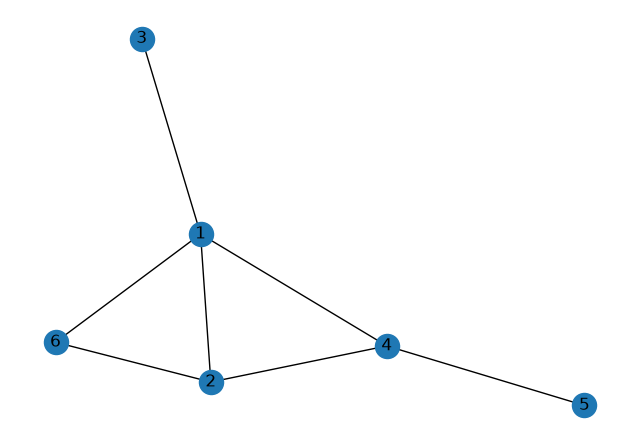
\includegraphics[width=10cm]{img/hw1/graph1}
\end{center}

\subsection{Part B}

The adjacency matrix is as follows:
\[\begin{pmatrix}
        0 & 1 & 1 & 1 & 1 & 1 \\
        1 & 0 & 0 & 0 & 1 & 0 \\
        1 & 1 & 0 & 0 & 1 & 0 \\
        0 & 0 & 1 & 0 & 0 & 0 \\
        0 & 1 & 0 & 0 & 0 & 1 \\
        1 & 0 & 0 & 0 & 1 & 0
    \end{pmatrix}\]
and its corresponding network looks like this:
\begin{center}
    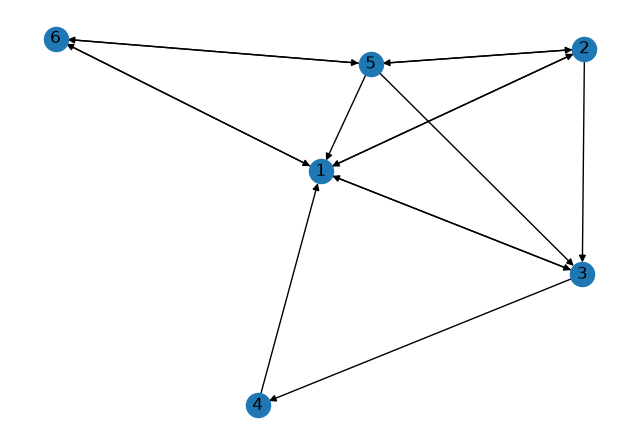
\includegraphics[width=10cm]{img/hw1/graph2}
\end{center}

\section{Problem 5}

\subsection{Part A}

BWOC let there be a 3-regular graph with $2k+1$ nodes.

The number of edges must be both an integer and equal to $\frac{3(2k+1)}{2}$
since every node is connected to three others.

However, these two conditions contradict each other, as $3(2k+1)$ is always odd. $\square$

\subsection{Part B}

A tree with $n$ nodes must have $n-1$ edges.

Since there's $n-1$ edges, the sum of the node degrees is $2(n-1)$.
This makes the average degree $\frac{2(n-1)}{2} < 2$. $\square$

\section{Problem 6}

\begin{enumerate}
    \item The adjacency matrix of $G_1$ is
          \[\begin{pmatrix}
                  0 & 0 & 0 & 0 & 1 & 1 \\
                  1 & 0 & 0 & 0 & 0 & 0 \\
                  0 & 1 & 0 & 0 & 0 & 0 \\
                  1 & 0 & 1 & 0 & 0 & 0 \\
                  0 & 0 & 0 & 1 & 0 & 0 \\
                  0 & 0 & 1 & 0 & 1 & 0
              \end{pmatrix}\]
    \item The incidence matrix of $G_2$ is
          \[\begin{pmatrix}
                  1 & 1 & 0 & 0 & 0 & 0 \\
                  0 & 1 & 1 & 0 & 1 & 0 \\
                  0 & 0 & 0 & 1 & 1 & 1 \\
                  0 & 0 & 0 & 0 & 0 & 1
              \end{pmatrix}\]
    \item I'll use the adjacency list representation:
          \begin{center}
              \begin{tabular}{ c|c }
                  \hline
                  Node & Neighbors  \\
                  \hline
                  1    & 2          \\
                  2    & 1, 3, 5    \\
                  3    & 2, 5       \\
                  4    & 5, 6       \\
                  5    & 2, 3, 4, 6 \\
                  6    & 4, 5       \\
                  \hline
              \end{tabular}
          \end{center}
    \item I ran this code:
          \begin{python}
import matplotlib.pyplot as plt
import networkx as nx

incoming = [
    [],
    [5, 6],
    [1],
    [2],
    [1, 3],
    [4],
    [3, 5]
]

g = nx.Graph()
for to, from_ in enumerate(incoming):
    for f in from_:
        g.add_edge(f, to)

pos = nx.circular_layout(sorted(g.nodes()))
nx.draw(g, pos=pos, with_labels=True)
plt.show()
          \end{python}
          To get this result:
          \begin{center}
              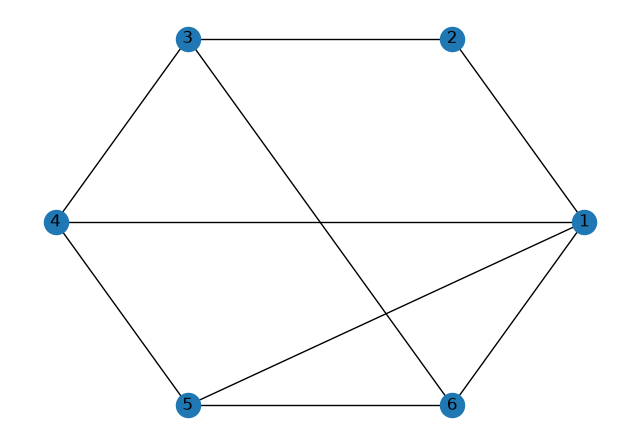
\includegraphics[width=10cm]{img/hw1/graph3}
          \end{center}
          It's rotated and reflected a bit, but this is indeed the undirected
          version of $G_1$.
\end{enumerate}

\section{Problem 7}

An hour, maybe an hour and a half?
I don't really keep track of these kinds of things.

\end{document}
